% !TeX root = RJwrapper.tex
\title{Understanding pandoc lua filters}
\author{by Abhishek Ulayil}

\maketitle

\abstract{
pandoc supports intermediate modification of the Abstract Syntax Tree (AST) between
the parsing and writing phase using filters. This supplement paper highlights
the use cases of such filters written in the Lua language on LaTeX, markdown and native AST.
}

\section{Introduction}
To fully understand pandoc filters, one must first grasp the document conversion process. A document in one format is read/parsed into an intermediate form, known as an abstract syntax tree (AST). A document writer is a specialized type-setter to read an AST and produce the contents in the chosen article format. Converting markdown to HTML, for example, will entail these pandoc operations. Figure~\ref{fig:workflow} shows the conversion workflow within pandoc.

\begin{figure}[htbp]
  \centering
  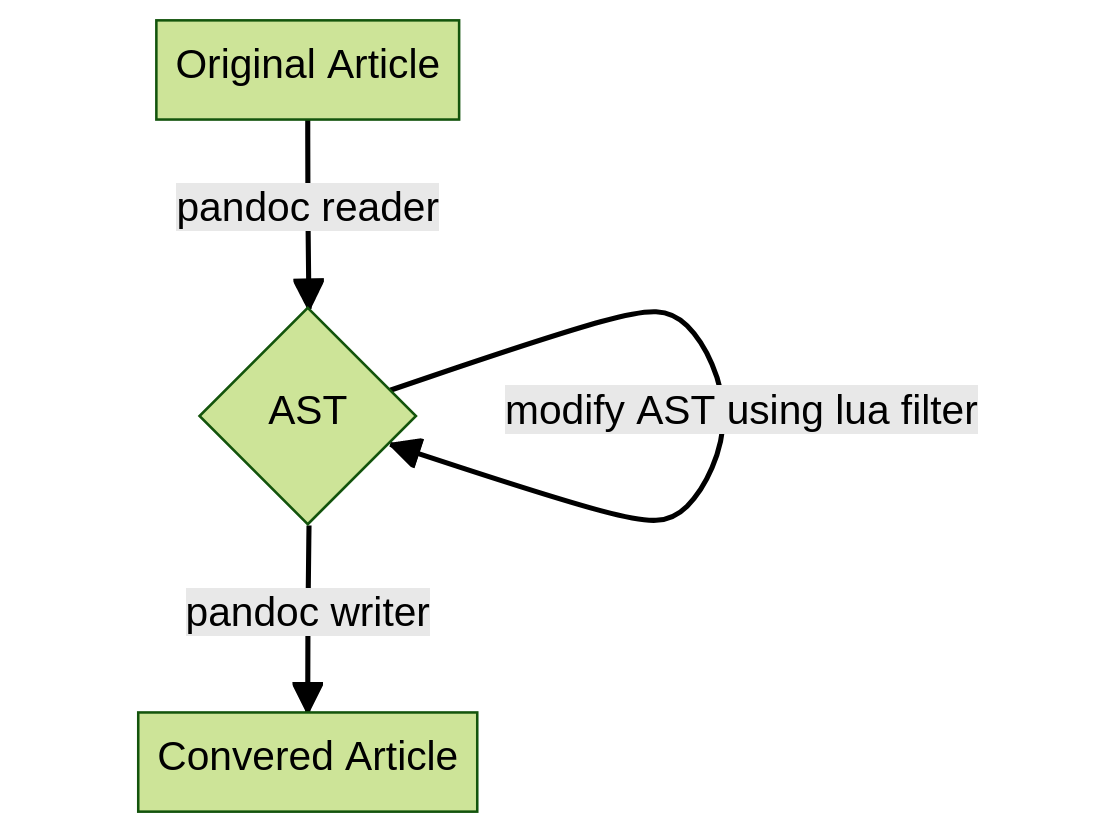
\includegraphics[width=0.6\textwidth]{figures/workflow.png}
  \caption{Conversion workflow.}
  \label{fig:workflow}
\end{figure}

When specific elements require adjustment, the Lua filters enter the picture. Assume you're converting markdown to HTML and want the page to have automated numbering for figures or tables. 
If you use markdown, there is no system for automatically numbering figures/tables; to retain 1:1 conversion, the HTML output will also lack numbering. 

At this point, you might wish there was a way to add such a feature. Then there is the possibility of unlimited choices for customization, including every customization as an option in pandoc or the writer is not viable. 
To address this, the idea of filters emerged, with which you could modify the AST before the writer could read it to obtain the desired result \citep{pandocfilters}.

\section{Need of Lua filters}

Continuing the example above, let's create a dummy article, where we need to add
numbering. One way could be to keep a counter of images, and add a prefix \verb|"Figure X :"|
to each figure caption. This will serve the purpose of numbering the images in the end result.

\begin{verbatim}
![R logo](Rlogo-5.png){width="10%"}

![penguins](penguins.png){width="15%"}

\end{verbatim}

\begin{figure*}[htbp]
\begin{verbatim}
pandoc example.md --from markdown --to html5 --output example.html
\end{verbatim}
\caption{pandoc command without lua filter or extensions.}
\label{code:2}
\end{figure*}

Now if we convert the above markdown file to HTML5 using the pandoc command in Figure~\ref{code:2}, we get Figure~\ref{fig:1}.


\begin{figure*}[!htbp]
\centering
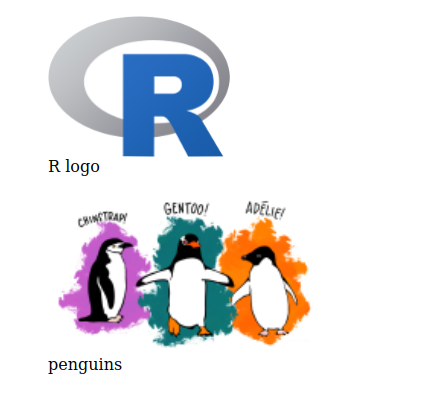
\includegraphics[width=0.5\linewidth]{figures/example.png}
\caption{Vanilla HTML5 output.}
\label{fig:1}
\end{figure*}

As we can see, there is no figure numbering done automatically, which is generally
the expected result. If we want to include numbering, we would need
to write a Lua filter. This Lua filter will modify the AST and make the changes we 
desire.

We call a Lua filter in the pandoc command show in Figure~\ref{code:2} using the \verb| --lua-filter name_of_filter.lua|
option in pandoc.

In the next section we write a Lua filter to manipulate the figures in Figure~\ref{code:3}.

\section{Writing pandoc Lua filters}

\begin{figure}[htbp]
\begin{verbatim}
figures = 0
is_fig = 0

function Figure(el)
      local label = ""
      pandoc.walk_block(el,{ Image = function(el)
                     is_fig = 1
                     end})
      if is_fig == 1 then
	        figures = figures + 1
	        label = "Figure " .. tostring(figures) .. ":"
      end
	    local caption = el.caption
	    if not caption then
          caption = {pandoc.Str(label)}
    	else
          caption = {pandoc.Str(label),pandoc.Space()}
    	end
    	el.caption.long[1].content = caption .. el.caption.long[1].content
    	is_fig = 0
    	return el
end
\end{verbatim}
\caption{A Lua filter to add figure numbering.}
\label{code:3}
\end{figure}

Everything in Lua revolves around tables; for example, the pandoc AST or the document is one giant table with sub-tables.

In pandoc, there are two sorts of elements: \verb|Blocks| and \verb|Inlines|. \verb|Blocks| are complicated constructions constructed from simple pieces (\verb|Inlines|). A \verb|Para|, for example, is a \verb|Block| made up of several \verb|Str| \verb|Inlines|.

The first step in writing a filter is to select a target type, that is, which \verb|Block| or \verb|Inline| this filter will target.
Following the selection, we name the function after the target type and each element in the argument as \verb|el|.
For instance, in the case of our filter, it would be \verb|function Figure(el)|. Pandoc is smart enough to match the names of filter functions to the AST elements.

Now within the filter function we can assume that \verb|el| will contain the table object of a Figure element from the document. We can use many functions over it or \verb|Inlines| contained in it. One such function to walk over all the elements inside the block is \verb|walk_block|. Walk functions are a great way to check or count the presence of certain elements in a block. We use \verb|walk_block| to check if there are any \verb|Image| inline elements within the \verb|Figure| block. This is because after pandoc 3 \citep{pandoc} \verb|Figure| blocks can now contain elements other than \verb|Images| as well.

If there is an \verb|Image| then we append \verb|"Figure X :"| to the caption of the \verb|Figure| element.
and return the modified element.

\section{Interpreting changes using Lua filters}

The filter in Figure~\ref{code:3} when included in the pandoc command will generate Figure~\ref{fig:2} 
using the command in Figure~\ref{code:4}.

\begin{figure}[htbp]
\begin{verbatim}
pandoc example.md --from markdown --to html5 --output filtered-example.html
--lua-filter image_numbering_filter.lua
\end{verbatim}
\caption{pandoc command with Lua filter.}
\label{code:4}
\end{figure}

\begin{figure}[htbp]
\centering
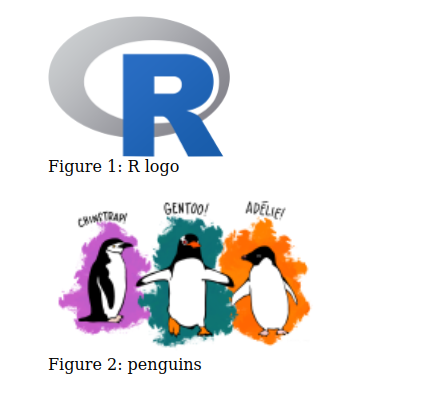
\includegraphics[width=0.5\linewidth]{figures/example-filtered.png}
\caption{HTML5 output with desired filtering.}
\label{fig:2}
\end{figure}

\section{Usage of pandoc lua filters in the \CRANpkg{texor} package}
Pandoc Lua filters are used in the \CRANpkg{texor} package to modify the AST for various markups.
 Table~\ref{tab:filters} summarizes the use of each filter.
\begin{table}
\begin{tabular}{|l|p{10cm}|}
\hline
File Name & Description\\
\hline
\verb|abs_filter.lua| & {Filters out unicode \verb|182| character.}\\
\hline
\verb|bib_filter.lua| & Clears out the bibliography from the article itself as it will be added to the metadata.\\
\hline
\verb|R_code.lua| & Adds a class component \verb|'r'| to CodeBlocks for code highlighting. \\
\hline
\verb|image_filter.lua| & Fixes extensions for image paths without an extension or with \verb|.pdf| extension. \\
\hline
\verb|table_caption.lua| & Adds table numbering in the captions similar to the ones found in R Markdown and \CRANpkg{kable}-based tables. \\
\hline
\verb|image_caption.lua| & Adds Figure/Algorithm/CodeBlock/WideTable numbering as well as clears out residuals of tikz/algorithm images. \\
\hline
\verb|conversion_compat_check.lua| & This filter keeps a count of all \verb|Inline| and \verb|Block| elements and writes it to a yaml file. \\
\hline
\verb|equation_filter.lua| & Adds \CRANpkg{bookdown} style equation numbering to LaTeX equation/math environments.\\
\hline
\verb|bookdown_ref.lua| & Changes the format of links to \CRANpkg{bookdown} (markdown) style.\\
\hline
\verb|issue_checker.lua| & Searches and notifies any occurrence of unrecognized math commands.\\
\hline
\verb|find_pdf_files.lua| & This filter creates a list for all image PDF files included in the article.\\
\hline
\end{tabular}
\caption{A summary of all Lua filters used in the \CRANpkg{texor} package (available in the \href{https://github.com/Abhi-1U/texor/tree/master/inst}{/inst} folder of the package).}
\label{tab:filters}
\end{table}





\begin{thebibliography}{2}
    \providecommand{\natexlab}[1]{#1}
    \providecommand{\url}[1]{\texttt{#1}}
    \expandafter\ifx\csname urlstyle\endcsname\relax
      \providecommand{\doi}[1]{doi: #1}\else
      \providecommand{\doi}{doi: \begingroup \urlstyle{rm}\Url}\fi

\bibitem[Krewinkel, Lucero (2023)]{pandoc}
A.~ Krewinkel and A.~ Lucero,
\newblock pandoc 3.0 Release notes,
\newblock \emph{pandoc} \penalty0 2023
\newblock URL \url{https://pandoc.org/releases.html}

\bibitem[MacFarlane and other pandoc authors (2023)]{pandocfilters}
John MacFarlane and other pandoc authors,
\newblock Pandoc Lua filters,
\newblock \emph{pandoc documentation} \penalty0 2023
\newblock URL \url{https://pandoc.org/lua-filters.html}

\end{thebibliography}


\address{%
Abhishek Ulayil\\
Student, Institute of Actuaries of India\\%
Mumbai, India\\
ORCiD: 0009-0000-6935-8690\\
}
